\documentclass[12pt,a4paper]{article}

% Font stuff
\usepackage{fontspec}

% lets use roboto because it is open and quite nice, or?
% \setmainfont{Roboto}[
%   Path           = ../fonts/,
%   Extension      = .ttf,
%   UprightFont    = *-Regular,
%   ItalicFont     = *-Italic,
%   BoldFont       = *-Bold,
%   BoldItalicFont = *-BoldItalic,
% ]

% Switch from babel to improve word wrapping etc with Swedish
%\usepackage[swedish]{babel}
\usepackage{polyglossia}
\setmainlanguage{swedish}

\usepackage[left=2.5cm,right=2.5cm,top=1.5cm,bottom=4cm]{geometry}
\setlength{\headheight}{82pt}

%% Important tex cmds
\usepackage{pdftexcmds}

\usepackage[document]{ragged2e}
% Mathptmx ruins unicode it seems
%\usepackage{mathptmx}
\usepackage{fancyhdr}
\usepackage{lastpage}
\usepackage{graphicx}
\usepackage{graphicx}
\makeatletter
\def\maxwidth{\ifdim\Gin@nat@width>\linewidth\linewidth\else\Gin@nat@width\fi}
\def\maxheight{\ifdim\Gin@nat@height>\textheight\textheight\else\Gin@nat@height\fi}
\makeatother
% Scale images if necessary, so that they will not overflow the page
% margins by default, and it is still possible to overwrite the defaults
% using explicit options in \includegraphics[width, height, ...]{}
\setkeys{Gin}{width=\maxwidth,height=\maxheight,keepaspectratio}
% Set default figure placement to htbp
\makeatletter
\def\fps@figure{htbp}
\makeatother
\usepackage{lipsum}
\usepackage[hidelinks]{hyperref}
\usepackage{longtable,booktabs}

\usepackage[compact]{titlesec}

% Include packages for mermaid etc
\usepackage{framed}

\providecommand{\tightlist}{%
  \setlength{\itemsep}{2pt}\setlength{\parskip}{0pt}\setlength{\partopsep}{2pt}\setlength{\topsep}{2pt}}

\renewcommand\labelitemi{--}

\setcounter{secnumdepth}{0}
\setlength{\parskip}{0.5cm}
\setlength{\parindent}{0.0mm}

\setcounter{tocdepth}{1}

\pagestyle{fancy}
\fancyhf{}

\lhead{\raisebox{-0.5\height}{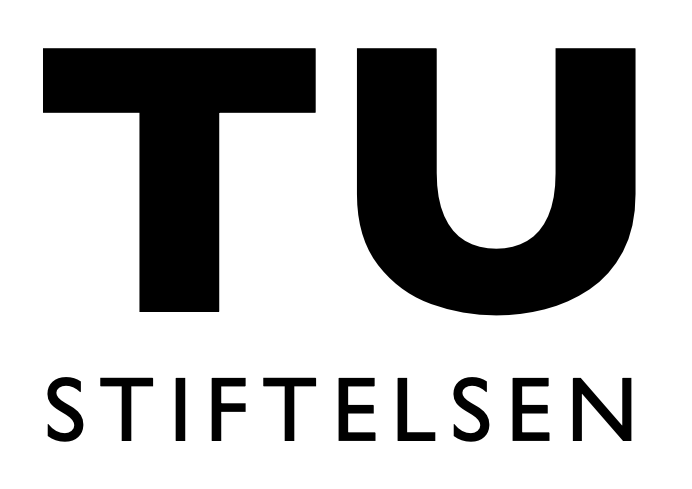
\includegraphics[width=3cm]{../template/tu-logo}}}

\chead{\raisebox{-0.6\height}{\parbox[b][][t]{5.5cm}{%
\begin{center}
\large
Kryptolåda
\end{center}}}}

\rhead{\begin{tabular}{rl}
Beteckning: & XYZ\\
Version: & 0.2\\
Datum: & 2024-02-27\\
Sida: & \thepage~av~\pageref{LastPage}
\end{tabular}}

\begin{document}

\section*{Kryptolåda}



\section{Inledning}\label{inledning}

Detta dokument beskriver en kryptolåda som kan sättas med utsida mot det
publika Internet (enligt Internetspecifikationen) och på sin insida
erbjuda paketförmedling enligt Internetspecifikationen med trafikskydd
och textskydd.

En kryptolåda ska givet en paketförmedlingstjänst enligt
Internetspecifikationen kunna hitta andra kryptolådor för att upprätta
relevanta koppel.

\subsection{Bakgrund och syfte}\label{bakgrund-och-syfte}

Inom och mellan vissa organisationer finns fristående nätverk som är
baserade på internetteknologi, men logiskt skilda från internet.
Användningen av dem motiveras ofta med högre krav till tillgänglighet
och driftsäkerhet än vad som påstås vara möjligt med förbindelser över
internet. Två exempel på sådana nät är
\href{https://www.msb.se/sv/verktyg--tjanster/sgsi/}{SGSI} och
\href{https://www.inera.se/tjanster/alla-tjanster-a-o/sjunet/}{Sjunet}.
På grund av hur de fristående näten realiseras tekniskt kan de
paradoxalt nog ha fler felkritiska systemdelar (eng. single points of
failure) än motsvarande internetbaserade lösningar. Det kan exempelvis
bero på att de är beroende av en enda infrastrukturleverantörs tekniska
system, där de kan dela kablar, kopplingsutrymmen, nätverksutrustning
med mera med internet.

Kryptolådan ska göra det möjligt och enkelt att använda internet för
verksamhetskritisk kommunikation på ett sätt som överensstämmer med
internets arkitekturprinciper. Förbindelsen mellan två kryptolådor och
den information som skickas mellan dem ska skyddas med avseende
konfidentialitet, riktighet, tillgänglighet och äkthet enligt
nedanstående tabell.

\begin{longtable}[]{@{}
  >{\raggedright\arraybackslash}p{(\columnwidth - 2\tabcolsep) * \real{0.5000}}
  >{\raggedright\arraybackslash}p{(\columnwidth - 2\tabcolsep) * \real{0.5000}}@{}}
\toprule\noalign{}
\begin{minipage}[b]{\linewidth}\raggedright
Egenskap
\end{minipage} & \begin{minipage}[b]{\linewidth}\raggedright
Beskrivning
\end{minipage} \\
\midrule\noalign{}
\endhead
\bottomrule\noalign{}
\endlastfoot
Konfidentialitet & Den överförda informationen skyddas mot obehörig
avlyssning genom kryptering. \\
Riktighet & Den överförda informationen skyddas mot avsiktlig och
oavsiktlig förändring. \\
Tillgänglighet & Systemdesignen ska, så långt det är tekniskt möjligt,
skydda mot avsiktliga försök att påverka tillgängligheten i kryptolådan
och bakomliggande (skyddade) system. \\
Äkthet & Kryptolådan ska endast förmedla trafik från behöriga avsändare
till bakomliggande (skyddade) system. \\
\end{longtable}

Utöver funktionaliteten i ett vanligt VPN-krypto ska kryptolådan klara
överbelastningsattacker (DOS-attacker) med en trafikmängd motsvarande
full linjehastighet på lådans internetsida. (I skrivande stund upp till
400~Gbps.) Projektet saknar budget att skapa en produkt. Inledningsvis
ska en specifikation tas fram. Specifikationen ska gå att använda för
att ta fram ett proof-of-concept.

\subsection{Avhängighet}\label{avhuxe4ngighet}

Detta dokument är beroende av Internetspecifikation.

\subsection{Begrepp}\label{begrepp}

\begin{itemize}
\tightlist
\item
  \textbf{DoS-skydd:} Denial-of-service skydd från trafik som kommer
  från det publika Internet. En del av trafikskyddet.
\item
  \textbf{Trafikskydd:} Ibland benämnt \emph{signalskydd}, rör skydd av
  trafikflöden och behandlar bland annat störsändningar, falska
  meddelanden, och hoppande frekvenser / mottagaradresser.
\item
  \textbf{Textskydd:} Ofta benämnt som kryptering, rör att skydda
  meddelandeinnehållet även om en antagonist kan läsa trafiken.
\end{itemize}

\section{Arkitektur}\label{arkitektur}

Övergripande hanterar arkitekturen för kryptolåda krypterad end-to-end
trafik mellan två godtyckligt valda platser på Internet. Se
\hyperref[arkitektur]{arkitekturskiss} för exempelritning av
arkitekturen.

\begin{figure}
\centering
\includesvg[width=0.5\textwidth,height=\textheight]{skiss.svg}
\caption{Arkitekturskiss}
\end{figure}

En kryptolåda kan både skicka och ta emot paket. Inkommande paket ska
vara adresserade till kryptolådan

Tunnelidentiteter består av en kombination av:

\begin{itemize}
\tightlist
\item
  protokoll
\item
  mottagaradress (IPv6)
\item
  mottagarport
\end{itemize}

TODO: Vad är begärandet av en ny adress en del av? Använder vi bara
prefix från Internetspecifikationen och växlar mellan dem, eller ska vi
lägga till hur man begär nya adresser via DHCP-PD eller en hel
BGP-snurra?

TODO: Vem begär ny tunnelidentitet? Ska vi ha en kontrollenhet / annat
som har ansvar att upprätthålla tunnlar osv.

TODO: Mesh, vilken del beslutar om hur vi bygger vårt mesh?

TODO: Kontrollplan?

\subsection{Funktionalitet}\label{funktionalitet}

Användare som vill koppla samman IPv6-nätverk på ett sätt som uppfyller
ovan nämnda säkerhetskrav kan använda kryptolådan. Lådans kryptotextsida
ansluts till internet och tilldelas en /64-adressrymd. Lådans
klartextsida ansluts till en router på det interna (skyddade) nätverket.
Kryptolådan tillhandahåller en lager 2-anslutning till klartextsidan på
en eller flera andra kryptolådor. Över den anslutningen kan de anslutna
routrarna skicka godtycklig trafik, inklusive routinginformation.

Konfidentialitet, riktighet och äkthet i trafiken tillses genom
kryptering med en lämplig autentiserad symmetrisk kryptoalgoritm
(\href{https://en.wikipedia.org/wiki/ChaCha20-Poly1305}{ChaCha20-Poly1305}?)
I det enklaste användningsfallet har två kryptolådor en delad hemlighet
som används för att generera en sessionsnyckel med t.ex.
\href{https://en.wikipedia.org/wiki/HKDF}{HKDF}. Sekvensnumrering
används för att detektera återuppspelningsattacker.

\subsubsection{Skydd mot
överbelastningsattacker}\label{skydd-mot-uxf6verbelastningsattacker}

Systemen på kryptolådans klartextsida skyddas mot
överbelastningsattacker genom den autentiserade krypteringen.

En överbelastning av kryptolådan kommer emellertid få effekten att alla
system som skyddas av den blir otillgängliga. För att skydda mot detta
använder kryptolådan sig av hoppande adresser. Med ett visst intervall
(typiskt sett något hundratal millisekunder) byter kryptolådan adress.
Intervallet kan vara en systemparameter eller förhandlas mellan två
lådor i samband med sessionsinitieringen, t.ex. genom mätning av RTT.

Paket till andra destinationsadresser än nuvarande eller närmast
föregående adress kastas. För att kunna genomföra en
överbelastningsattack som mättar kryptolådans förmåga att dekryptera
meddelanden måste en motståndare kunna sniffa äkta trafik från en annan
kryptolåda och ställa om sin överbelastningstrafik till den nya adressen
inom något hundratal millisekunder.

Kryptolådan använder statistiska metoder för att identifiera
källadresser som skickar stora mängder obehörig trafik och använder
\href{https://datatracker.ietf.org/doc/rfc9244/}{DDoS Open Threat
Signaling (DOTS)} för att tillse att trafiken filtreras så tidigt så
möjligt i nätverket.

Adresshoppningen kan exempelvis realiseras genom att de 64 lägsta
bitarna i output från AES(\emph{k}, \emph{CT}), där k är en nyckel
genererad från del delade hemligheten mellan två kryptolådor och
\emph{CT} är klartexten genererad enligt tabellen nedan.

\begin{longtable}[]{@{}
  >{\raggedright\arraybackslash}p{(\columnwidth - 4\tabcolsep) * \real{0.3333}}
  >{\raggedright\arraybackslash}p{(\columnwidth - 4\tabcolsep) * \real{0.3333}}
  >{\raggedright\arraybackslash}p{(\columnwidth - 4\tabcolsep) * \real{0.3333}}@{}}
\toprule\noalign{}
\begin{minipage}[b]{\linewidth}\raggedright
Bit
\end{minipage} & \begin{minipage}[b]{\linewidth}\raggedright
Data
\end{minipage} & \begin{minipage}[b]{\linewidth}\raggedright
Förklaring
\end{minipage} \\
\midrule\noalign{}
\endhead
\bottomrule\noalign{}
\endlastfoot
0-15 & Låd-id & Anger kryptolådans id. Medger upp till 65536 kryptolådor
med samma nyckel. \\
16-56 & Reserv & Ej specificerade. Sätts till noll eller till ett
slumpmässigt värde som handskakas fram. \\
57-83 & Adressintervall (ms) & Giltighetstiden för en adress enligt
systemparameter eller handskakning. \\
84-100 &
\href{https://en.wikipedia.org/wiki/Julian_day\#Variants}{Modified
Julian Date} & Antal hela dagar sedan midnatt den 17 november 1858
(\href{https://en.wikipedia.org/wiki/Coordinated_Universal_Time}{UTC}). \\
101-127 & Tid sedan midnatt (ms) & Början på adressens giltighetstid
(UTC). \\
\end{longtable}

Ett alternativ till att använda låd-id är att förhandla fram en separat
nyckel för varje riktning vid handskakningen. Kryptolådorna måste ha
gemensam tid med en noggrannhet som är signifikant bättre än
adressintervallet. Den föreslås erhållas genom
\href{https://datatracker.ietf.org/doc/html/rfc8915}{NTS}. Användning av
MJD och tid sedan midnatt eliminerar problem med skottsekunder,
UNIX-epochs osv.

\subsection{Nödvändiga
systemparametrar}\label{nuxf6dvuxe4ndiga-systemparametrar}

\begin{itemize}
\tightlist
\item
  Tilldelat /64-nät på kryptotextsida
\item
  Tilldelat /64-nät för motparternas kryptotextsidor (strikt taget
  endast nödvändigt för ena parten i en tvåvägsförbindelse)
\item
  Delad hemlighet (en per motpart)
\item
  Adressintervall
\item
  Adress till NTS-server (och certifikatkedja)
\item
  DOTS-parametrar
\end{itemize}

\subsection{Proof-of-concept}\label{proof-of-concept}

Ett fungerande proof of concept ska minst ha följande funktionalitet: *
Sessionsinitiering över förbindelsen med hjälp av delad hemlighet och
HKDF. * Krypterad och autentiserad överföring av data mellan
klartextsidorna på två kryptolådor. * Hoppande IPv6-adresser på
kryptotextsidan. * Filtrering av obehöriga paket med hjälp av
destinationsadress (adresshoppning) och autentiserad kryptering.

\subsection{Kvarvarande frågor och
observationer}\label{kvarvarande-fruxe5gor-och-observationer}

\begin{itemize}
\tightlist
\item
  Antalet samtidiga sessioner kommer att påverka prestandan. Det typiska
  användningsfallet kommer att vara en eller en handfull sessioner.
\item
  Ska kryptolådan erbjuda skydd mot trafikanalys (fyllnadssignalering)?
\item
  Hur hanteras out-of-order packets mht. sekvensnumreringen?
\item
  Är det nödvändigt att skicka
  \href{https://en.wikipedia.org/wiki/Neighbor_Discovery_Protocol}{NDP}-paket
  med nya adresser för att inte få packet loss vid adresshoppningen? Hur
  lång tid innan adressbyte i så fall?
\item
  Kan vi ta bort gamla adresser ur neighbortabellen med NDP?
\item
  När måste man byta nyckel för adresshoppningen? Även om man har
  observerat en viss adress så är sannolikheten \emph{nästan} lika stor
  att den dyker upp igen. Med tanke på hur ofta/sällan de byts så borde
  det räcka något decennium eller så, men det borde kontrollräknas.
\item
  Beskriv någon hyfsat effektiv statistisk metod för att identifiera
  källadresser som skickar stora mängder överbelastningstrafik. (För det
  är inte praktiskt genomförbart att hålla en lista på alla i minnet.)
\end{itemize}

\subsection{DoS-skydd}\label{dos-skydd}

Denial-of-service skyddet ska se till att kryptolådan ej kan sättas ur
funktion genom designade trafikströmmar. Detta görs genom att
kryptolådor ska klara av ett fullt trafikflöde enligt dess
datalänklager.

TODO: Givet korrekt protokoll, port och adress så lämnar DoS över till
trafikskydd?

\begin{itemize}
\tightlist
\item
  \textbf{Krav:}

  \begin{itemize}
  \tightlist
  \item
    DoS-skyddet \textbf{ska} filtrera bort all trafik som inte är
    adresserad till aktiv kryptografisk tunnel.
  \item
    DoS-skyddet \textbf{ska} upprätthålla full tillgänglighet vid
    datalänkslagrets fulla trafikhastighet.
  \end{itemize}
\end{itemize}

\subsection{Trafikskydd}\label{trafikskydd}

TODO: Vad gör trafikskyddet i den här lösningen?

TODO: De flesta protokoll idag gör en kombo av trafikskydd och
textskydd. Vill vi dela upp dem? Antar att det finns fördelar med att
kunna dela upp dem även fast de flesta implementationer sköter trafik
och textskydd tillsammans.

\begin{itemize}
\tightlist
\item
  \textbf{Krav:}

  \begin{itemize}
  \tightlist
  \item
    Trafikskyddet \textbf{ska} meddela DoS-skyddet aktiva
    tunnelidentiteter.
  \end{itemize}
\end{itemize}

\subsection{Textskydd}\label{textskydd}

TODO: Hur mycket valfrihet ska finnas för textskyddet? Får användare
välja vad som helst?

\begin{itemize}
\tightlist
\item
  \textbf{Krav:}

  \begin{itemize}
  \tightlist
  \item
    Textskyddet \textbf{ska} meddela trafikskyddet aktiva
    tunnelidentiteter.
  \end{itemize}
\end{itemize}

\section{Exempel}\label{exempel}

\subsection{Från klient på insidan till trafik på
utsidan}\label{fruxe5n-klient-puxe5-insidan-till-trafik-puxe5-utsidan}

TODO: Reffa internetspecifikationen. På insidan så ska en klient inte se
någon skillnad.

\begin{figure}
\centering
\includesvg[width=1\textwidth,height=\textheight]{inut.svg}
\caption{Trafik som går från klient}
\end{figure}

\subsection{Trafik utifrån in till
klient}\label{trafik-utifruxe5n-in-till-klient}

TODO: Hur sker avskalning av skydd?

\section{Verifikation}\label{verifikation}

TODO: Ta fram mätbara krav på kryptolådan

\section{Proof of concept}\label{proof-of-concept-1}

TODO: Ta fram PoC? Ev raspberry pi / liten referensdesign som man kan
bygga och testa?

\section{Annat}\label{annat}

TODO: Hur hanterar vi kvantsaker? Ex nyckelutbyte över annan rutt än
Internet?

\section{Från tidigare spec}\label{fruxe5n-tidigare-spec}

\subsection{Frequency hopping}\label{frequency-hopping}

Kan man använda de sista 64-bitarna i en IPv6-adress för frequency
hopping på ett bra sätt?

Vilket sliding window behöver vi för att hoppa effektivt?

\subsection{Kryptosystem}\label{kryptosystem}

För de användare som tidigare använt fasta förbindelser eller någon form
av VPN-tjänst tillhandahåller Fem små hus-infrastrukturen ett
kryptosystem. Kryptosystemet ger skydd mot obehörig trafik, avlyssning
och överbelastningsattacker.

Kryptosystemets princip är att det överför Ethernet-paket mellan två
punkter genom att man kapslar in det krypterade Ethernet-paketet i ett
IPv6-paket som skickas över infrastrukturen. Olika metoder används för
att skydda kryptots ändpunktsadresser mot överbelastningsattacker. Har
man flera korresponderande motparter via samma krypto identifieras de
med ett VLAN per motpart.

Kryptot ansluts till infrastrukuren med 100/400Gbit och tjänsten mot
användaren är förmedling av Ethernet-paket med 100/10Gbit-anslutning.
Maximal överförd lager 2-Ethernet-MTU är 8210 byte.

För detaljspecifikation av kryptot, se del 4 som tas fram av en separat
arbetsgrupp.

En enklare form av tunnling, motsvarande MPLS, är att använda L2TPv3
över IPv6. Funktionaliteten finns i de flesta kommersiella routrar och
kan i vissa fall kombineras med routerns kryptofunktion.
\end{document}
